% -*- LaTeX -*-
% -*- coding: utf-8 -*-
%
% ~~~~~~~~~~~~~~~~~~~~~~~~~~~~~~~~~~~~~~~~~~~~~~~~~~~~~~~~~~~~~~~~~~~~~~~~~~~~~~
%
%                             michael a.g. aïvázis
%                      california institute of technology
%                      (c) 1998-2010  all rights reserved
%
% ~~~~~~~~~~~~~~~~~~~~~~~~~~~~~~~~~~~~~~~~~~~~~~~~~~~~~~~~~~~~~~~~~~~~~~~~~~~~~~
%

\lecture{}{20100120}

% --------------------------------------
% threads and shared memory parallelism 
\begin{frame}[fragile]
%
  \frametitle{Threads and shared memory parallelism}
%
  \begin{itemize}
%
  \item recall the shared memory architecture
%
    \begin{figure}
      \centering
      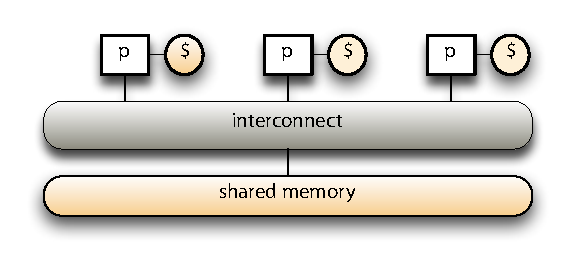
\includegraphics[scale=0.5]{figures/shared-memory.pdf}
    \end{figure}
    \vspace{-1.0em}
%
    \begin{itemize}
    \item processors are connected to a memory pool with a global address space
    \item processors have their own cache but no private memory
    \end{itemize}
%
  \item model is relevant for {\em threads}
%
    \begin{itemize}
    \item lightweight processes that can be scheduled independently, but share many OS
      resources
      \begin{itemize}
      \item CPU
      \item memory
      \item but also file descriptors, process environment, etc.
      \end{itemize}
    \item supported by most modern operating systems
    \end{itemize}
%
  \end{itemize}
%
    \begin{figure}
      \centering
      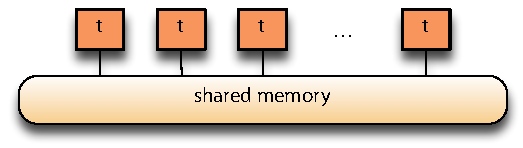
\includegraphics[scale=0.5]{figures/threads-memory.pdf}
    \end{figure}
%
\end{frame}

% --------------------------------------
% template
\begin{frame}[fragile]
%
  \frametitle{Processes and threads}
%
  \begin{itemize}
%
  \item in most operating systems, a process has
    \begin{itemize}
    \item process id and group id, user id and group id
    \item environment variables
    \item working directory
    \item scheduling information
    \item registers, stack, heap, instruction stream
    \item file descriptors, signal handlers, other process dependent structures
    \end{itemize}
%
  \item threads 
    \begin{itemize}
      \item share many of the per-process properties
        \begin{itemize}
        \item they are lightweight since they incur low overhead
        \end{itemize}
      \item have their own copy of
        \begin{itemize}
        \item registers, stack, instruction stream
        \item scheduling information
        \end{itemize}
    \end{itemize}
%
  \item threads are important programming constructs
    \begin{itemize}
    \item every vendor supports a proprietary interface
    \item {\em pthreads}, the POSIX standard API specification brought portability
    \item standardized creation, management, synchronization
    \end{itemize}
%
  \end{itemize}
%
\end{frame}

% --------------------------------------
% template
\begin{frame}[fragile]
%
  \frametitle{The pthreads API}
%
  \begin{itemize}
%
  \item threads require support from the compiler, the linker, the loader, and the OS kernel
    \begin{itemize}
    \item thread safety
    \end{itemize}
%
  \item special command line argument to most compliant compilers
    \begin{itemize}
    \item changes the instruction strategy
    \item adds the pthread runtime library to the link line
    \item links against the thread safe runtime
    \end{itemize}
%
  \item naming conventions
    \begin{table}
      \scriptsize
      \centering
      \begin{tabular}{l|l}
        Prefix & Functional group\\ \hline
        {\tt pthread\_ } &
            access to the threads, and some miscellaneous routines\\
        {\tt pthread\_attr\_ } & 
            thread attribute objects\\
        {\tt pthread\_mutex\_ } & 
            mutexes\\
        {\tt pthread\_mutexattr\_ } & 
            mutex attribute objects\\
        {\tt pthread\_cond\_ } & 
            condition variables\\
        {\tt pthread\_condattr\_ } & 
            condition variable attribute objects\\
        {\tt pthread\_key\_ } & 
            thread-specific data keys\\
        {\tt pthread\_rwlock\_ } & 
            read/write locks\\
        {\tt pthread\_barrier\_ } & 
            synchronization barriers\\
      \end{tabular}
    \end{table}
%
  \item the standard specifies the API for \CC\ only; \fortran\ support varies
    \begin{itemize}
    \item must include \srcfile{pthread.h}
    \end{itemize}
%
  \item lots of good books; see \href{http://acm114.caltech.edu/references}
%
  \end{itemize}
%
\end{frame}

% --------------------------------------
% template
\begin{frame}[fragile]
%
  \frametitle{Creating threads}
  \begin{itemize}
%
  \item create threads by calling
%
  \begin{C}
int pthread_create(
    pthread_t* id, const pthread_attr_t* attr,
    void* (*startup)(void*), void* arg);
  \end{C}
%
\item initially a process has one thread; every other thread must be explicitly created
  by calling \function{pthread\_create} and passing
  \begin{itemize}
  \item \identifier{id}: the location where a unique thread identifier will be stored
  \item \identifier{attr}: an opaque attribute object with thread initialization options
  \item \function{startup}: a pointer to a \CC\ function that will be executed by the thread
    once it gets scheduled
  \item \identifier{arg}: user defined data to be passed to \function{startup}; may be \NULL
  \end{itemize}
%
  \item once scheduled, threads are first class citizens
%
  \item the maximum number of threads per process depends on the implementation
%
  \end{itemize}
%
    \begin{figure}
      \centering
      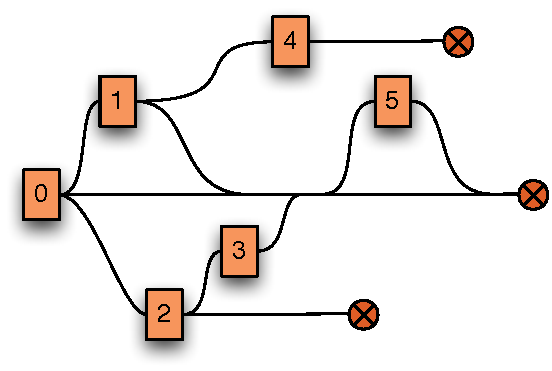
\includegraphics[scale=0.5]{figures/threads.pdf}
    \end{figure}
%
\end{frame}

% --------------------------------------
% terminating threads
\begin{frame}[fragile]
%
  \frametitle{Terminating threads}
%
  \begin{itemize}
%
    \item several ways to terminate a thread
      \begin{itemize}
      \item the thread returns from \function{main}
      \item the thread explicitly calls \function{pthread\_exit}
      \item the thread is killed when another thread calls \function{pthread\_cancel}
      \item the process terminates due to some system call, e.g.~\function{exit},
        \function{exec}, etc.
      \end{itemize}
%
  \item use \function{pthread\_exit} to kill a thread when it is no longer needed
%
    \begin{C}
int pthread_exit(void * status);
    \end{C}
%
  \item if \function{main} finishes and any threads remain
    \begin{itemize}
    \item they get killed unless \function{main} has called \function{pthread\_exit}
    \item otherwise they continue to run
    \end{itemize}
%
  \item thread routines do not have to call \function{pthread\_exit} unless they intend to pass
    their termination status to their creator
%
  \item \function{pthread\_exit} does not perform any process cleanup: it doesn't flush/close
    files, release other resources, signal the process parent, etc.
  \end{itemize}
%
\end{frame}

% --------------------------------------
% hello world
\begin{frame}[fragile]
%
  \frametitle{Hello world}
  \label{slide:hello-world}
%
  \begin{C}
#include <pthread.h>
#include <stdio.h>
#define THREADS 10

void* hello(void* threadID) {
    long id = (long) threadID;
    printf("hello from %02ld/%0d\n", id, THREADS);
    pthread_exit(NULL);
    return NULL;
}

int main(int argc, char* argv[]) {
    long id;
    int status;
    pthread_t threads[THREADS];

    for (id=0; id<THREADS; id++) {
        printf("creating thread %02ld\n", id);
        status = pthread_create(&threads[id], NULL, hello, (void*) id);
        if (status) {
            printf("error %d in pthread_create\n", status);
        }
    }

    pthread_exit(NULL);
    return 0;
}
  \end{C}
%
\end{frame}

% --------------------------------------
% joining and detaching threads
\begin{frame}[fragile]
%
  \frametitle{Joining and detaching}
%
  \begin{itemize}
%
  \item in the example in \slideref{hello-world}, the main thread exits without knowing whether
    any of the threads it spawned have finished
    \begin{itemize}
    \item saying ``hello'' is asynchronous
    \item but gathering the results of parallel calculations normally isn't
    \end{itemize}
%
  \item {\em thread synchronization} can be achieved using \function{pthread\_join}
    \begin{itemize}
      \item the \function{pthread\_create} caller saves the thread id
      \item the thread is scheduled, executes, and calls \function{pthread\_exit}
      \item any other thread can wait for this thread to finish by calling
        \function{thread\_join} with the saved thread id and also retrieve the termination
        status
    \end{itemize}
%
  \item for this to work, a thread must be {\em joinable}
    \begin{itemize}
    \item controlled by the thread creation attributes
    \item for portability, you should always mark your joinable threads explicitly
    \end{itemize}
%
%
    \item a thread that will never be joined may be {\em detached}
      \begin{itemize}
      \item by setting the corresponding attribute during thread creation
      \item or, by calling \function{pthread\_detach} at any point
      \item detaching a thread saves some system resources
      \end{itemize}
        
  \end{itemize}
%
\end{frame}

% --------------------------------------
% mutexes
\begin{frame}[fragile]
%
  \frametitle{Creating mutexes}
%
  \begin{itemize}
%
  \item a {\em mutex} is a locking mechanism that helps guarantee exclusive access to a section
    of code, most often to control access to shared variables
%
  \item mutexes are created using
%
    \begin{C}
int pthread_mutex_init(
    pthread_mutex_t* mutex, const pthread_mutexattr_t* attr);
    \end{C}
%
    \begin{itemize}
    \item they start out unlocked
    \item the \identifier{attr} enables more advanced (but perhaps non-portable) use
    \end{itemize}
%
  \item mutexes are destroyed using
%
    \begin{C}
int pthread_mutex_destroy(pthread_mutex_t* mutex);
    \end{C}
%
    \begin{itemize}
    \item destroy mutexes you are no longer using to prevent resource leakage
    \end{itemize}
%
  \end{itemize}
%
\end{frame}

% --------------------------------------
% mutex manipulation
\begin{frame}[fragile]
%
  \frametitle{Locking and unlocking mutexes}
%
  \begin{itemize}
%
  \item threads manipulate mutexes through
%
    \begin{C}
int pthread_mutex_lock(pthread_mutex_t* mutex);
int pthread_mutex_trylock(pthread_mutex_t* mutex);
int pthread_mutex_unlock(pthread_mutex_t* mutex);
    \end{C}
%
  \item \identifier{pthread\_mutex\_lock} attempts to gain exclusive access
    \begin{itemize}
    \item if the mutex is unlocked, it locks it and returns
    \item otherwise, it blocks until the mutex is unlocked; when the mutex is unlocked, it
      locks it and returns
    \end{itemize}
%
  \item \identifier{pthread\_mutex\_unlock} attempts to release a mutex
    \begin{itemize}
    \item if it was previously locked by this thread, the mutex is unlocked
    \item if it was not previously locked, the call returns with an error code
    \item if it was locked, but not by the calling thread, the call returns an error code
    \end{itemize}
%
  \item \identifier{pthread\_mutex\_trylock} attempts to lock the mutex
    \begin{itemize}
    \item if it is unlocked, the call locks it and returns
    \item if it is locked, the call returns immediately with a {\em busy} error code
    \end{itemize}
%
  \item locking and unlocking mutexes is explicitly orchestrated by the programmer
  \item when multiple threads are blocked waiting for a mutex, there is no way to predict which
    one will succeed when the mutex becomes available
%
  \end{itemize}
%
\end{frame}

% --------------------------------------
% condition variables
\begin{frame}[fragile]
%
  \frametitle{Condition variables}
%
  \begin{itemize}
%
  \item condition variables build upon mutexes to enable threads to signal each other when some
    condition is met
%
  \item they are created using
%
    \begin{C}
int pthread_cond_init(
    pthread_cond_t* condition, const pthread_condattr_t* attr);
    \end{C}
%
  \item and destroyed using
%
    \begin{C}
int pthread_cond_destroy(pthread_cond_t* condition);
    \end{C}
%
  \end{itemize}
%
\end{frame}

% --------------------------------------
% using condition variables
\begin{frame}[fragile]
%
  \frametitle{Using condition variables}
%
  \begin{itemize}
%
  \item the following three routies implement the condition variable semantics
%
    \begin{C}
int pthread_cond_wait(pthread_cond_t* cond, pthread_mutex_t* mutex);
int pthread_cond_signal(pthread_cond_t* cond);
int pthread_cond_broadcast(pthread_cond_t* cond);
    \end{C}
%
  \item \identifier{pthread\_cond\_wait} blocks the calling thread until the specified
    condition is {\em signaled}
    \begin{itemize}
    \item it must be called with the mutex locked by the calling thread
    \item \identifier{pthread\_cond\_wait} releases the lock while the thread is blocked
    \item after the matching signal is received, the thread is awakened and the mutex locked
    \item the thread is responsible for releasing the mutex when it is done
    \end{itemize}
%
  \item \identifier{pthread\_cond\_signal} wakes up a thread that is waiting for the given
    condition variable
    \begin{itemize}
    \item mutex must be locked before calling it
    \item mutex must be unlocked after signaling, so blocking threads can be awakened
    \end{itemize}
%
  \item \identifier{pthread\_cond\_broadcast} can be used instead if multiple threads are
    waiting for a signal
%
  \end{itemize}
%
\end{frame}

% --------------------------------------
% condition variable caveats
\begin{frame}[fragile]
%
  \frametitle{Condition variable caveats}
%
  \begin{itemize}
%
  \item be careful with condition variables; make sure that
    \begin{itemize}
    \item a thread has called \identifier{pthread\_cond\_wait} before any thread
      calls \identifier{pthread\_cond\_signal}
    \item the mutex associated with the condition is locked before calling
      \identifier{pthread\_cond\_wait}, otherwise it might {\em not block}
    \item the thread that calls \identifier{pthread\_cond\_signal} unlocks the associated
      mutex, otherwise the threads waiting for the signal will continue to block
    \end{itemize}
%
%
  \end{itemize}
%
\end{frame}

% --------------------------------------
% the attribute interface
\begin{frame}[fragile]
%
  \frametitle{Attributes of threads, mutexes and condition variables}
%
  \begin{itemize}
%
  \item threads, mutexes and condition variables have associated attribute structures that can
    be used to tune the default creation parameters
%
  \item they are created and destroyed using
%
    \begin{C}
int pthread_attr_init(pthread_attr_t* attr);
int pthread_attr_destroy(pthread_attr_t* attr);

int pthread_mutexattr_init(pthread_mutexattr_t* attr);
int pthread_mutexattr_destroy(pthread_mutexattr_t* attr);

int pthread_condattr_init(pthread_condattr_t* attr);
int pthread_condattr_destroy(pthread_condattr_t* attr);
    \end{C}
%
  \item typically, the defaults are adequate and tuned to the details of the operating system
%
  \item if you make excessive use of the stack, e.g.~large arrays as local variable or deep
    recursion, you might want to know about
%
    \begin{C}
int pthread_attr_getstacksize(pthread_attr_t* attr, size_t* size);
int pthread_attr_setstacksize(pthread_attr_t* attr, size_t size);
    \end{C}
%
  \end{itemize}
%
\end{frame}

% --------------------------------------
% miscellaneous
\begin{frame}[fragile]
%
  \frametitle{Other useful routines}
%
  \begin{itemize}
%
  \item a thread can access its unique id assigned by the system by calling 
%
    \begin{C}
pthread_t pthread_self(void);
    \end{C}
%
  \item since system thread ids are opaque types, you cannot use \operator{==} to compare
    them; instead, use
%
    \begin{C}
int pthread_equal(pthread_t id1, pthread_t id2);
    \end{C}
%
  \item you can place all thread initialization code in a startup routine and call
%
    \begin{C}
int pthread_once(pthread_once_t* control_structure, void (*startup_routine)(void));
    \end{C}
%
  \end{itemize}
%
\end{frame}

% --------------------------------------
% template
\begin{frame}[fragile]
%
  \frametitle{Advanced topics}
%
  \begin{itemize}
%
  \item there is quite a bit more in the standard
%
  \item {\em keys}: creating and accessing per-thread data
    \begin{itemize}
    \item as the code get more complicated, it becomes increasingly difficult to pass complete
      thread-specific information from function to function
    \item possible solutions:
      \begin{itemize}
      \item the \fortran\ syndrome, where subroutines end up having dozens of arguments
      \item global variables
      \item an associative container that allows each thread to store and retrieve arbitrary
        data
      \end{itemize}
%
    \end{itemize}
%
    \item finer control over thread scheduling
      \begin{itemize}
      \item scheduling algorithms and priorities are implementation dependent
      \item there are routines in the standard that enable explicit tuning
      \item the standard guarantees that the routines will be {\em available}, but they don't
        have to be {\em implemented}
      \end{itemize}
%
    \item condition variable sharing across processes
%
    \item explicitly canceling threads
%
    \item the somewhat complicated interactions between threads and signals
%
    \item other synchronization constructs: barriers and read/write locks
%
  \end{itemize}
%
\end{frame}

% end of file 
